\clearpage
\section{Introduction to the Robot-maze Environment}

The coursework exercises for this year's CS118 course will be based on 
a simulated `robot-maze' environment.  A small robot has been designed to
be able to navigate its way through mazes to find a target at some given
location.  This task resembles those used in the classic learning 
experiments of the 1960s which included laboratory
mice (and cheese, mild electric shocks, mice of the opposite sex, etc).
The objective of the robot (or mouse as it was then) is to 
find the given target as rapidly and efficiently as
possible, learning the maze over several runs and so on.  

Building a real robot and a real maze requires a combination of efficient 
sensors and mechanics, sophisticated steering and speed control, clever 
maze exploration and navigation procedures and, no doubt, a good deal of
glue.  For the purpose of these exercises we focus
entirely on designing the maze exploration and navigation algorithms.
We make no attempt to model the physics of a moving wheeled (or legged!)
robot and concentrate solely on the part of the 
problem which can best be solved with software. 

\subsection{The robot-maze environment}

The simulated Robot-maze environment has the following characteristics:

\begin{itemize}

\item The robot moves through a simple square-block maze of the type
  illustrated in Figure~\ref{maze}.  The floor space of the maze is divided
  into squares of uniform size.  Each square is either occupied by a
  wall or is empty.

\item The robot occupies exactly one non-wall square and moves in
  discrete steps, one square at a time, north, south, east, or west.
  The robot cannot move diagonally.  If the robot attempts to move
  outside the boundary of the maze or into squares occupied by walls it
  suffers a harmless collision (indicated by flashing red in the
  simulation) and stays in the same square.

\item The direction the robot moves in is determined by the way it 
  is facing (its heading, 
  indicated by an arrow in the simulation).  The robot can change
  the direction it is facing by rotating on the spot.
  Each of these rotations are directed by the robot's control procedure
  -- a method called {\tt controlRobot} -- which is run once before the 
  robot makes a move. 

\item A robot run \emph{usually} begins at the top left-hand
  square of the maze.  The run ends when either the robot reaches the
  target or the user loses patience and stops the robot manually
  (by pressing {\bf Reset}).
  The target square is usually the bottom right-hand corner of the maze,
  but this along with the robot start position can be modified by the 
  user. 

\end{itemize}

\begin{figure}
\centering
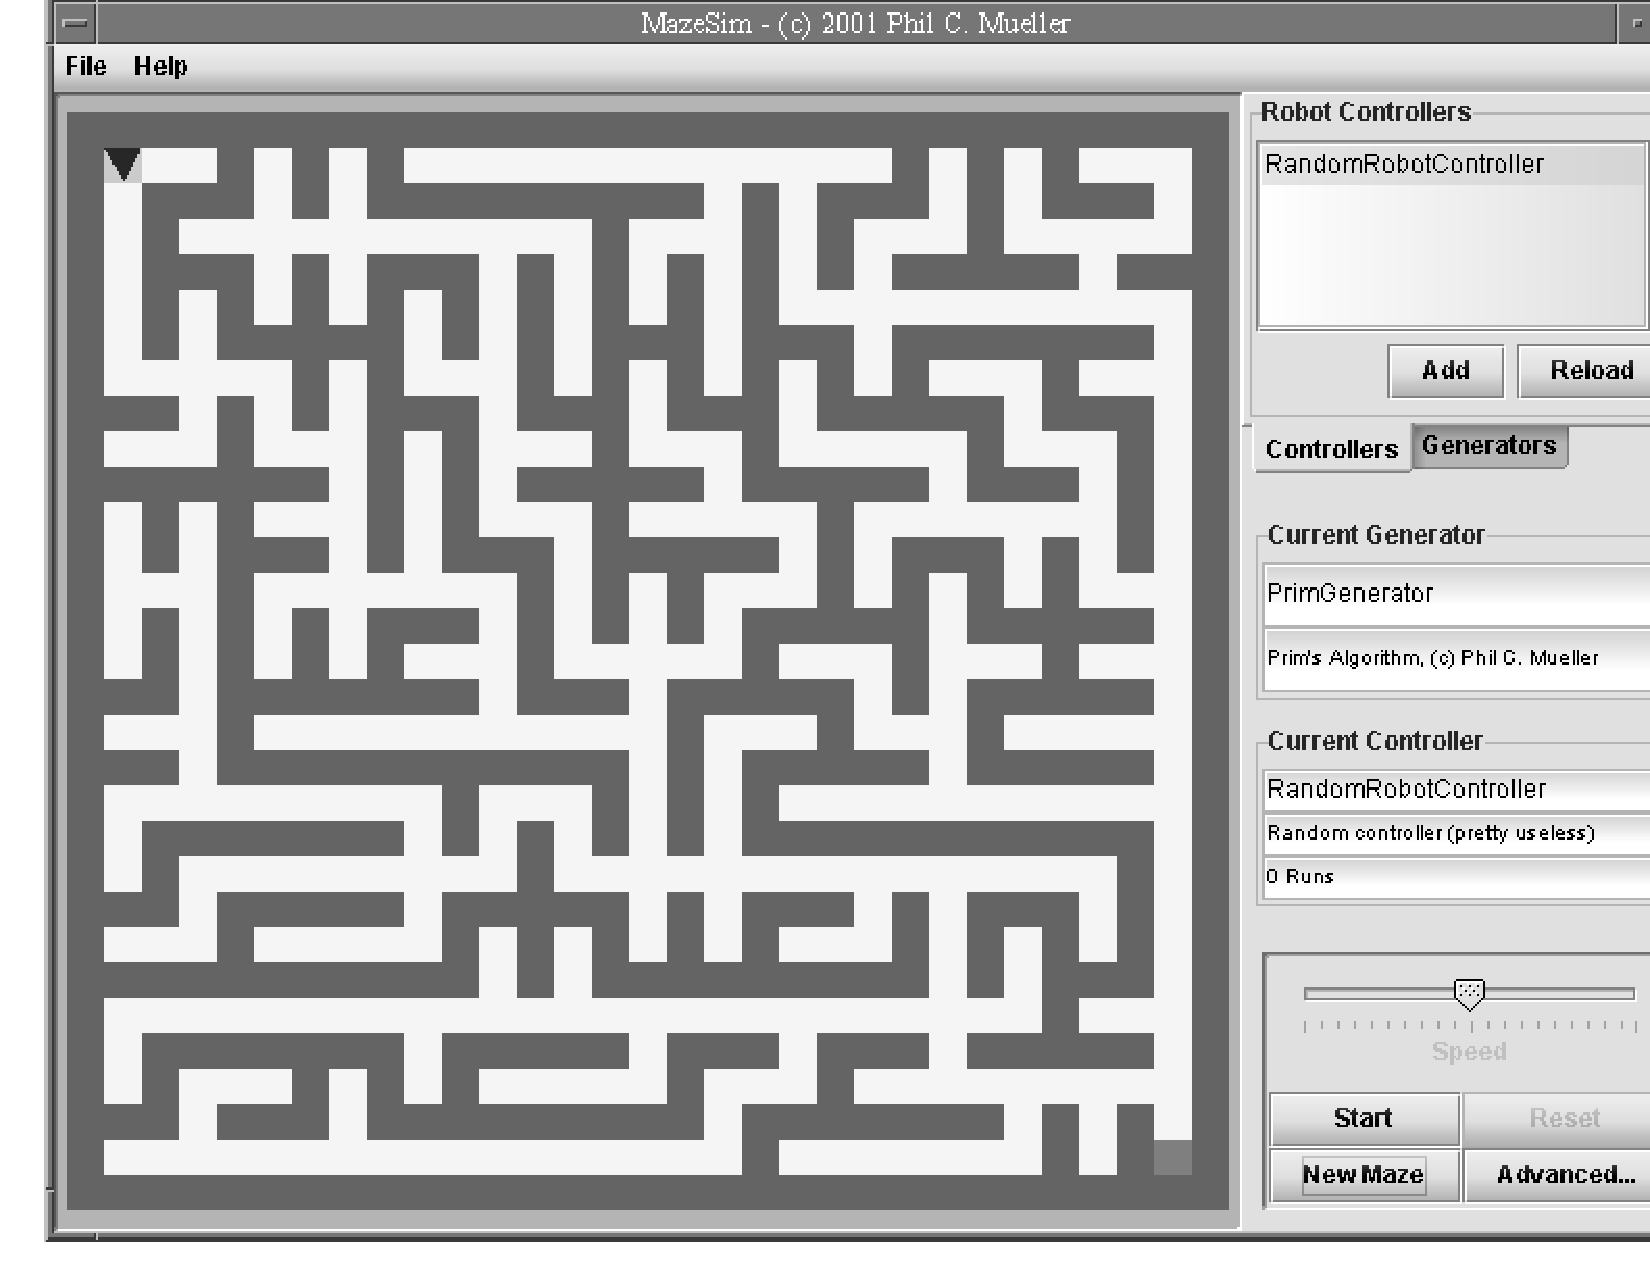
\includegraphics[width=10cm]{maze.pdf}
\caption{The Robot-maze environment\label{maze}}
\end{figure}

During its execution the robot's control program (which you are required to
write) has access to the following information:

\begin{itemize}

\item The direction the robot is currently facing;

\item The status of the squares ahead, behind, left and to the right of the
  robot.  Squares are either walls, empty, or beenbefore squares which are 
  empty squares the robot
  has previously occupied during its current run through the maze.  The
  boundaries of the maze are treated as walls;

\item The {\it x} and {\it y} co-ordinates of the square the robot is currently
  occupying, and those of the target square;

\item How many attempts the robot has made at solving the given maze.

\end{itemize}


\subsection{Programming robot control programs}

The simulated robot-maze environment is written in Java. The programs which 
you are required to write for this course are also Java based which means 
that you will be writing code which directly hooks into this robot-maze
environment. \\

\noindent
To allow this hook-up, there needs to be a common interface between the 
robot-maze Java code and your own Java code. Essentially this means that 
you need to be talking the same language; we define this language below.\\

\noindent
The information listed below is important and you should make sure that you 
understand what it all means. If you are not clear on anything then you 
might like to talk about it between yourselves. Understanding {\em 
program interfaces} like this is very important, particularly if you are to 
use it to write your own program code.

\subsubsection{Specifying headings in the maze}

Four pre-defined constants are used to specify directions in the
maze.  These are \\

{\tt NORTH, EAST, SOUTH, WEST} \\

\noindent
where the maze follows the usual mapping convention of having {\tt NORTH} 
upwards and {\tt EAST} to the right etc. \\

\noindent
These elements of the interface 
language are concretely represented as Java {\tt int} values. This will 
be useful to know when you start referring to the types of these values in
your programs. One advantage of this scheme is that \\

{\tt NORTH+1 = EAST}; {\tt EAST+1 = SOUTH}; {\tt SOUTH+1 = WEST}.

\subsubsection{Specifying directions relative to the robot heading}

Four pre-defined constants are used to specify directions
relative to the robot's heading. \\

{\tt LEFT, RIGHT, AHEAD, BEHIND}\\

\noindent
As with headings these are also of the type {\tt int} and therefore \\

{\tt AHEAD+1 = RIGHT}; {\tt RIGHT+1 = BEHIND}; {\tt BEHIND+1 = LEFT} \\

\noindent
A fifth constant {\tt CENTRE} is also defined, which can be useful as a
`null' or `give-up' value when communicating values between parts of
complex control programs.\\

\noindent
Do not be put off by the fact that these values have an {\tt int} type.
As far as the control
programmer (this is you) is concerned, all references to headings and
directions are done using the constant {\em name} (i.e. {\tt RIGHT}, 
{\tt NORTH} etc.) 
and not the constant {\em value} used to represent it. This is our first
encounter with {\em program abstraction}. \\

\noindent
As the values are defined as part of a Java interface,
we need to prefix these values with the name of the interface when they are
used in the actual program code. The interface is called {\tt IRobot} and 
therefore any reference to the constant {\tt AHEAD} in the code is in fact 
done using {\tt IRobot.AHEAD}. This might seem a bit quirky but you will 
soon get used to it. 


\subsubsection{Sensing the squares around the robot}
\label{lookmethod}

The method {\tt robot.look(}{\em direction}{\tt )} takes a value
specifying a direction relative to the robot (e.g. {\tt IRobot.AHEAD} or {\tt
IRobot.LEFT} etc.) and returns a value which indicates the state of the
corresponding square neighbouring the robot. The possible states are\\

{\tt IRobot.PASSAGE, IRobot.WALL, IRobot.BEENBEFORE}\\

\noindent
{\tt IRobot.PASSAGE} indicates an empty square that has not yet been 
visited on the
current run through the maze. {\tt IRobot.BEENBEFORE} indicates an empty 
square that
has already been visited during the current run through the maze. {\tt
IRobot.WALL} indicates a wall or the edge of the maze.\\

\begin{figure}
\centering
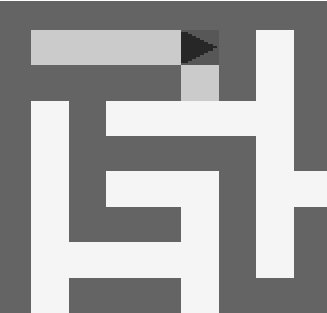
\includegraphics[width=2in]{mousemove}
\caption{Example of sensing robot surroundings\label{sensing}}
\end{figure}

\noindent
Figure~\ref{sensing} shows a typical situation that might arise during a
robot run. 
The robot is located in the arrowed square, facing in the direction of
the arrow, with squares visited previously during the same run shaded
in grey. The walls are in black. In this situation
{\tt robot.look} would return the following values:

\begin{center}
\begin{tabular}{l l} \hline
Function call & Result \\ \hline
{\tt robot.look(IRobot.AHEAD)}  & {\tt IRobot.WALL} \\
{\tt robot.look(IRobot.BEHIND)} & {\tt IRobot.BEENBEFORE} \\
{\tt robot.look(IRobot.LEFT)}   & {\tt IRobot.WALL} \\
{\tt robot.look(IRobot.RIGHT)}  & {\tt IRobot.BEENBEFORE} \\ \hline
\end{tabular}
\end{center}

\noindent
If the robot chooses to turn right and then move forward one square, 
then a call to the method {\tt robot.look(IRobot.AHEAD)} would
return {\tt IRobot.PASSAGE}.

\subsubsection{Sensing and setting the robot's heading}

The method {\tt robot.getHeading()} returns the robot's current heading
in the maze.
That is either {\tt IRobot.NORTH}, {\tt IRobot.SOUTH}, {\tt IRobot.EAST} or 
{\tt IRobot.WEST}. In the example in Figure~\ref{sensing} a call to the 
method {\tt robot.getHeading()} would return the value {\tt IRobot.EAST}.
There is a sister method called {\tt robot.setHeading(x)},
which can be used to set the robot's heading (where the parameter {\tt x} is 
one of {\tt IRobot.NORTH}, {\tt IRobot.SOUTH}, {\tt IRobot.EAST} or 
{\tt IRobot.WEST}).

\subsubsection{Sensing the location of the robot and target}

The method {\tt robot.getLocation()} returns a {\tt Point} object with two public
variable members. You can get the $x$ and $y$ co-ordinates of the robot in the maze from
the {\tt Point} class by accessing the {\tt x} and {\tt y} members of the instance
using {\tt robot.getLocation().x} and {\tt robot.getLocation().y}.  The top left square in the
maze is square (1,1).\\

\noindent
Similarly, the method {\tt robot.getTargetLocation()} can be used to return the $x$ and $y$
co-ordinates of the robot's target.

\subsubsection{Specifying turns}

The method {\tt robot.face(}{\em direction}{\tt )} makes the robot turn
 in the {\em direction} specified (one of {\tt IRobot.AHEAD}, {\tt IRobot.BEHIND}, 
{\tt IRobot.LEFT}, or {\tt IRobot.RIGHT}) relative to its current heading.  
The turn is
 performed immediately and will be reflected in the results of
 subsequent calls to {\tt robot.getHeading()}.

\subsubsection{Moving the robot}

The control software which you will build is polled. This means that the 
code you write will be called by the robot-maze environment each time it is
ready to move the robot. This effectively switches control between 
the environment and your controller, and the environment and your 
controller, and the environment and your controller etc. \\

\noindent
The code which you write should therefore point the robot in a suitable 
direction. After the completion of your polled controller, the robot will automatically
advance in the direction the robot is facing\footnote{This is a change from previous years,
where your controller would advance the robot manually. If your controller points the robot at a wall,
when the environment advances, the robot will cause a collision with the wall.}.

\subsubsection{Generating random numbers}

The Java method {\tt Math.random()} returns a random floating point number 
greater than or equal to $0.0$ and less than $1.0$. The number
returned is computed so as to ensure that every number appears with
equal probability. \\

\noindent
To generate random numbers (almost!) uniformly distributed
between $0$ and $n$ you will need to take the result, multiply it by $n$, 
round it to the nearest integer (using {\tt Math.round()}), and then  
cast the result to an {\tt int} value, e.g. \\

{\tt int result = (int) Math.round(Math.random()*n);} \\

\noindent
So, the code \\

{\tt randno = (int) Math.round(Math.random()*3);} \\

\noindent
for example, will assign a random integer value between 0 and 3 inclusive 
(that is one of four distinct possibilities) to the variable {\tt randno}.

\subsubsection{Detecting the start of a run and a change of maze}


The method {\tt robot.getRuns()} returns a number ({\tt int}) which 
corresponds to the the number of previous runs which the robot has made 
on a given maze.  
After you have run a robot through a maze you will notice that the current
controller screen to the right of the robot-maze environment displays 
{\tt 1 Run}. This is the result of the {\tt robot.getRuns()} method. 
You will find that this method is useful in the second coursework.




